% ****** Start of file aapmsamp.tex ******
%
%   This file is part of the AAPM files in the AAPM distribution for REVTeX 4-2.
%   Version 4.2a of REVTeX, January 2015
%
%   Copyright (c) 2015 American Association of Physicists in Medicine (AAPM).
%
%   See the AAPM README file for restrictions and more information.
%
% TeX'ing this file requires that you have AMS-LaTeX 2.0 installed
% as well as the rest of the prerequisites for REVTeX 4.2
%
% It also requires running BibTeX. The commands are as follows:
%
%  1)  latex  aapmsamp
%  2)  bibtex aapmsamp
%  3)  latex  aapmsamp
%  4)  latex  aapmsamp
%
% Use this file as a source of example code for your aapm document.
% Use the file aapmtemplate.tex as a template for your document.
\documentclass[%
 aapm,
 mph,%
 amsmath,amssymb,
%preprint,%
 reprint,%
%author-year,%
%author-numerical,%
]{revtex4-2}
\usepackage{amssymb}
\usepackage{graphicx}
\usepackage{hyperref}
\usepackage{listings}
\usepackage{mathtools}
\usepackage{maple}
\usepackage[utf8]{inputenc}
\usepackage[svgnames]{xcolor}
\usepackage{amsmath}
\usepackage{breqn}
\usepackage{textcomp}
\usepackage{subcaption}
\usepackage[settings]{markdown}


% \begin{document}
\lstset{basicstyle=\ttfamily,breaklines=true,columns=flexible}
\pagestyle{empty}
\DefineParaStyle{Maple Bullet Item}
\DefineParaStyle{Maple Heading 1}
\DefineParaStyle{Maple Warning}
\DefineParaStyle{Maple Heading 4}
\DefineParaStyle{Maple Heading 2}
\DefineParaStyle{Maple Heading 3}
\DefineParaStyle{Maple Dash Item}
\DefineParaStyle{Maple Error}
\DefineParaStyle{Maple Title}
\DefineParaStyle{Maple Ordered List 1}
\DefineParaStyle{Maple Text Output}
\DefineParaStyle{Maple Ordered List 2}
\DefineParaStyle{Maple Ordered List 3}
\DefineParaStyle{Maple Normal}
\DefineParaStyle{Maple Ordered List 4}
\DefineParaStyle{Maple Ordered List 5}
\DefineCharStyle{Maple 2D Output}
\DefineCharStyle{Maple 2D Input}
\DefineCharStyle{Maple Maple Input}
\DefineCharStyle{Maple 2D Math}
\DefineCharStyle{Maple Hyperlink}


\usepackage{gensymb}
\usepackage{graphicx}% Include figure files
\usepackage{dcolumn}% Align table columns on decimal point
\usepackage{physics}
% \usepackage{mathtools}
% \usepackage{amsmath}
\usepackage{bm}% bold math
\usepackage[mathlines]{lineno}% Enable numbering of text and display math
\usepackage{multirow}
\usepackage[normalem]{ulem}
\useunder{\uline}{\ul}{}
\modulolinenumbers[5]% Line numbers with a gap of 5 lines

\begin{document}
\noindent
\header{ENGR 120}
%\preprint{AAPM/123-QED}

\title[]{\underline{Fluid Mechanics: Lab 5} \\
Venturi and Orfice flow measurements and characterization}.% Force line breaks with \\

\author{Christian Emil Lorentsen}%
\author{Serafin Stauch}
\author{Bryan Saldivar}
\author{Xuan Zhao}

\affiliation{University of California, Merced}
\date{\today}% It is always \today, today,
             %  but any date may be explicitly specified
\begin{abstract}
In this report we make use of accelerometers to determine flow rate through a pipe.

\end{abstract}

\maketitle
\linenumbers\relax % Commence numbering lines
\begin{quotation}
%Explain why the physics you are studying is interesting and relevant.
Venturi and Orifice meters provides and excellent way of measuring volume flow rate. From two simple pressure reading it is possible to measure the volume flow rate in a pipe using a Venturi meter, making it useful in a large variety of application. An Orifice meter also makes us able to measure the flow rate through a pipe, this time only using a small hole.

\end{quotation}
\section{\label{sec:level1}Background}
First, we look at the Venturi meter. It consists of a circular pipe, with a given volume flow rate. At a section of the pipe, where it conically shrinks shortly, we measure the pressure at three different points, see fig \ref{fig:Venturi}. The Orifice meter is almost identical to the Venturi meter, although there is no conical shrinkring, but a \textit{wall} with a small hole in the middle of diameter $d$, see fig \ref{fig:Orifice}.

\subsection{\label{sec:level2}Theory}
From Bernoullis eq. we get the following for the Venturi meter:

\begin{eqnarray}
P_a +\frac{1}{2} V_a^2 + \rho g z_a = p_b + \frac{1}{2} \rho V_b ^2 + \rho g z_1 \\
\Rightarrow A_b^2 P_V = \frac{1}{2}A_b^2 \rho \big(V_b^2 - \tfrac{d_a^4}{d_b^4}V_b^2 \big) 
\end{eqnarray}
Where we get $V_a = (d_b^2/d_a^2)V_b$ from conservation of mass. This leads to the following equations:
\begin{eqnarray}
    Q = \frac{\pi}{4}d_b^2 \sqrt{\frac{2P_v}{\rho(1-d_a^4/d_b^4)}} \\
    P_v = \frac{8Q^2\rho(1-d_a^4/d_b^4)}{\pi^2d_b^2}
    \label{eq:Qventuri}
\end{eqnarray}

Eq. 373\cite{White_Xue_2021}
\begin{equation}
    \bigg(\frac{p}{\gamma} + \frac{V^2}{2g} + z\bigg)_{in} = \bigg(\frac{p}{\gamma} + \frac{V^2}{2g} + z\bigg)_{out} + h_{friction}
\end{equation}
Since we have no pump or turbine. $z_{in}=z_{out}$ and applying between point A and B we get
\begin{eqnarray}
    h_{f1} = \frac{P_v}{\rho g} + \frac{1}{2g}(V_a^2-V_b^2) = \frac{P_v}{\rho g} + \frac{Q^2}{2gA_b^2}\bigg(\frac{d_b^4}{d_a^4}-1\bigg) \\
    = \frac{P_v}{\rho g} + \frac{2Q^2}{g\pi^2d_b^4}\bigg(\frac{d_b^4}{d_a^4}-1\bigg)
    \label{eq:hf1}
\end{eqnarray}
It is easy to apply it between point A an C, since they have the same crossectional area, and we loose the second term:
\begin{eqnarray}
    h_{f2} = \frac{P_d}{\rho g}
    \label{eq:hf2}
\end{eqnarray}
For the Orifice plate the relationship between the flow rate and pressure drop can be derived as \cite{White_2021}
\begin{eqnarray}
    Q = C_d A_t \bigg[\frac{2\Delta p}{\rho(1-\beta^4)}\bigg]
    \label{eq:Cd}
\end{eqnarray}
Where $C_d$ is the discharge coefficient, $A_t$ is the throat area and $\beta = d/D$, see fig \ref{fig:Orifice}
\subsection{\label{sec_level3}Method \& Setup}



We have a setup of pies consisting of three different materials: Copper, Galvanized Steel and PVC. We control the flow rate through the pipe, and take measurements at five different flow rates: $2, 3, 4, 6 m^3/hr$ and an unknown. For each flow rate, we have an accelerometer hooked up to the pipe, which measures the acceleration in 3 different directions $(x, y, z)$ for 30 seconds, and we take the mean of each. We then fit a linear model:

\begin{equation}
    y = A\cdot x + B
    \label{eq:linfunc}
\end{equation}

This model is run independently on all three axis, where we compare the $R^2$ for each model, to figure out which axis gives us the best results. We then process the data for the unknown results (take the mean) for the chosen axis and simply solve eq. \ref{eq:linfunc}:

\begin{equation}
    Flowrate = \frac{a-B}{A}
\end{equation}
Where $a$ is the mean acceleration and $A$ and $B$ are the  parameters from the fit
For the uncertainties we get:
\begin{eqnarray}
    \delta Flowrate = \sqrt{ \bigg(\frac{1}{A}\bigg)^2 (\delta a^2 + \delta B^2) + \bigg(\frac{a-B}{A^2}\bigg)^2 \delta A^2}
    \label{eq:Uncertainty}
\end{eqnarray}
Where $\delta A$ and $\delta B$ are found from the covariance matrix obtained by SciPy's curve\_fit function and $\delta a$ is found from the standard deviation of $a$:
\begin{eqnarray}
    \delta a = \frac{std(a)}{\sqrt{N}}
    \label{eq:deltaa}
\end{eqnarray}
Where $N$ is the number of data points for $a$.
\newpage
\section{DATA AND RESULTS}
\intput{Chapters/Results}


\subsection{Analysis}
If we were to (hypothetically) measure a pressure drop of $6.35 mbar$ across the orfice plate with $C_d \approx 0.363 m^{-1}$ you would get a volume flow rate of $Q\approx 9.80\cdot 10^{-6} m^3/s$
\begin{figure}[h!]
    \centering
    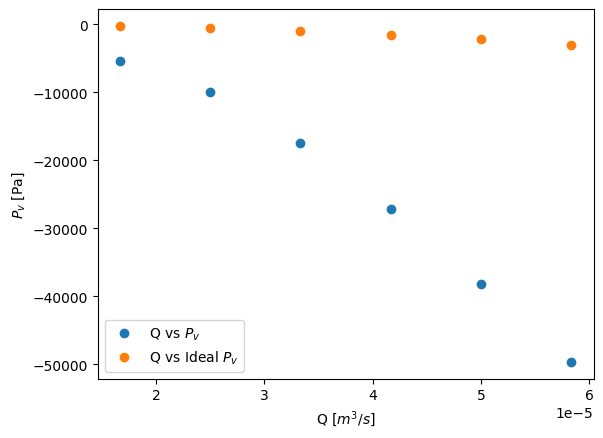
\includegraphics[width=60mm]{Diagrams/PvVsQ.png}
    \caption{Plot of measured $p_v$ vs $Q$ and and ideal $p_v$ vs $Q$}
    \label{fig:pvVsQ}
\end{figure}

\begin{table}[h!]
\resizebox{\columnwidth}{!}{%
\begin{tabular}{lr}
\toprule
h & Q \\
\midrule
$0.140 \pm 0.010$ & 0.00 \\
$0.160 \pm 0.010$ & 0.00 \\
$0.180 \pm 0.010$ & 0.00 \\
$0.190 \pm 0.010$ & 0.00 \\
$0.150 \pm 0.010$ & 0.00 \\
$0.190 \pm 0.010$ & 0.00 \\
\bottomrule
\end{tabular}

}
\caption{Table of calculated  \ref{eq:hf1} and \ref{eq:hf2}}
\label{table:hf1hf2}


\end{table}


\begin{figure}[h!]
    \centering
    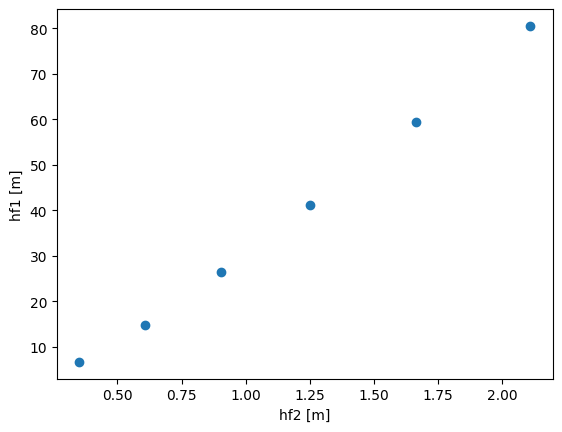
\includegraphics[width=60mm]{Diagrams/hf1Vshf2.png}
    \caption{Plot of $h_{f1}$ vs $h_{f2}$}
    \label{fig:hf1Vshf2}
\end{figure}


\begin{figure}[h!]
    \centering
    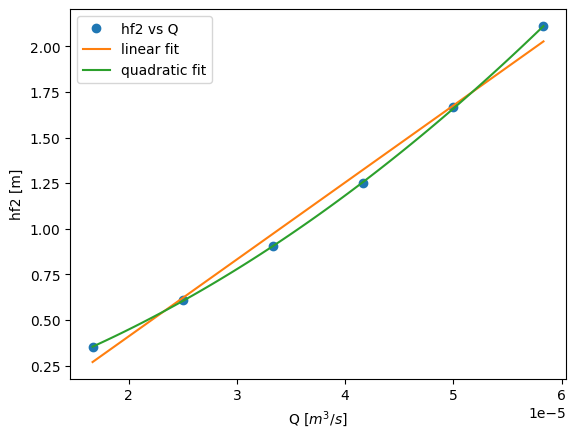
\includegraphics[width=60mm]{Diagrams/hf2VsQ.png}
    \caption{Plot of $h_{f2}$ vs $Q$ Including both linear $(a\cdot x+b)$ and quadratic fit$(a\cdot x^2 + b\cdot x^2 +c )$}
    \label{fig:hf2VsQ}
\end{figure}



\newpage
\section{DISCUSSION}
We observe that the results from table \ref{table:results} of  $(5.3\pm 3.3)m^3/hr$ for Copper, $(4.3\pm 2.9)m^3/hr$ for galvanized steel and $(6.2\pm 1.0)m^3/hr$ for PVC are quite similar, which is a good sign. Although, the uncertainties are quite high. This is likely due to the large standard deviation of $a$, as can be seen in the figures \ref{fig:copper}, \ref{fig:galvanized} and \ref{fig:PVC}. To get this lower you could either obtain more data (run the experiment longer) as seen in eq. \ref{eq:deltaa}. Another, probably better way is to train a more complex model, eg. a neural network or a generalised linear model and use more data, both in the form of running the expirement for longer and for more flow rates, althoguh depending on the applications, simple linear regression (as in this report) may be adequate.

\section{CONCLUSION}
In conclusion, we have effectively estimated flowrate throguh different pipes, obtaining the values $(5.3\pm 3.3)m^3/hr$ for Copper, $(4.3\pm 2.9)m^3/hr$ for galvanized steel and $(6.2\pm 1.0)m^3/hr$ for PVC. The uncertainties obtained are quite large, although depending on your application it may not be of issue. They can also be mitigated by obtaining more data ore training a more complex model.

{
\appendix
\section{Calculations}
\subsection{\label{app:python}Python code used to run the calculations and the numerical integration}
The calculations are done in python: (Code excluding plots)
\begin{lstlisting}[language = Python, caption = Python code]
import numpy as np
import matplotlib.pyplot as plt
from scipy.optimize import curve_fit

#Venturi
Q = np.array([1, 1.5, 2.0, 2.5, 3.0, 3.5])*10**(-3)/60
Pd = np.mean(np.array([[35,34], [61,58], [92,85],[ 125,120], [166,160], [209,204]])*10**2, axis = 1)
Pv = np.mean(np.array([[61, 46], [99, 100], [180,168], [272,272], [374,390], [493, 500]])*10**2, axis = 1)
da = 6.4*10**(-3)
db = 2.5*10**(-3)

IdealPv = (8*Q**2*(1-da**4/db**4))/(np.pi**2*db**4)


Qmeasured = np.pi/4 * db**2 * np.sqrt(2*9.81*(-Pv)/(998*(1-(da/db)**4)))
hf1 = Pv/(998*9.81) + 2*Q**2/(9.81*np.pi**2*db**4) * (da**4/db**4-1)
hf2 = Pd/(998*9.81)



def linfunc(x, a, b):
    return a*x + b

def quadfunc(x, a, b, c):
    return a*x**2 + b*x + c


parlin, covlin = curve_fit(linfunc, Q, hf2)
parquad, covquad = curve_fit(quadfunc, Q, hf2, p0 = [100,1,1])

X = np.linspace(np.min(Q), np.max(Q), 100)
Ylin = linfunc(X, *parlin)
Yquad = quadfunc(X, *parquad)



##Orifice
d = 4*10**(-3)
D = 6.4*10**(-3)    
At = np.pi/4 * (d)**2
beta = d/D
Q = np.array([1, 1.5, 2.0, 2.5, 3.0, 3.5])*10**(-3)/60
dP = np.mean(np.array([[18, 19], [40, 41], [75, 69], [114, 115], [165, 166], [232, 235]])*10**2, axis = 1)
Cd = Q/( At * np.sqrt(2*dP/(998*(1-beta**4))) )
print(Cd, "[m^3/s]")
print(np.mean(Cd))

dp = 6.35*10**2
Q = np.mean(Cd)*At*np.sqrt(2*dp/(998*(1-beta**4)))
print(Q)
\end{lstlisting}

}


\nocite{*}
\section*{\underline{Citations}}
\bibliography{aapmsamp}% Produces the bibliography via BibTeX.


\end{document}
%
% ****** End of file aapmsamp.tex ******
